\subsection{Inner detector}

The inner detector, as shown in figure~\ref{fig:inner_dec}, is the detector closest to beam pipe.
It's used to measure the position of charged particle tracks in high precision together with good momentum resolution,
among which the measurement of primary and secondary vertices and electron identification are especially important.
Due to the extremely high luminosity produced by the LHC, the precise measurements of vertex and momentum becomes tough and fine-granularity detectors are crucial.
The inner detector consists of three subdetectors described as below:
\begin{figure}[!htb]
  \centering
  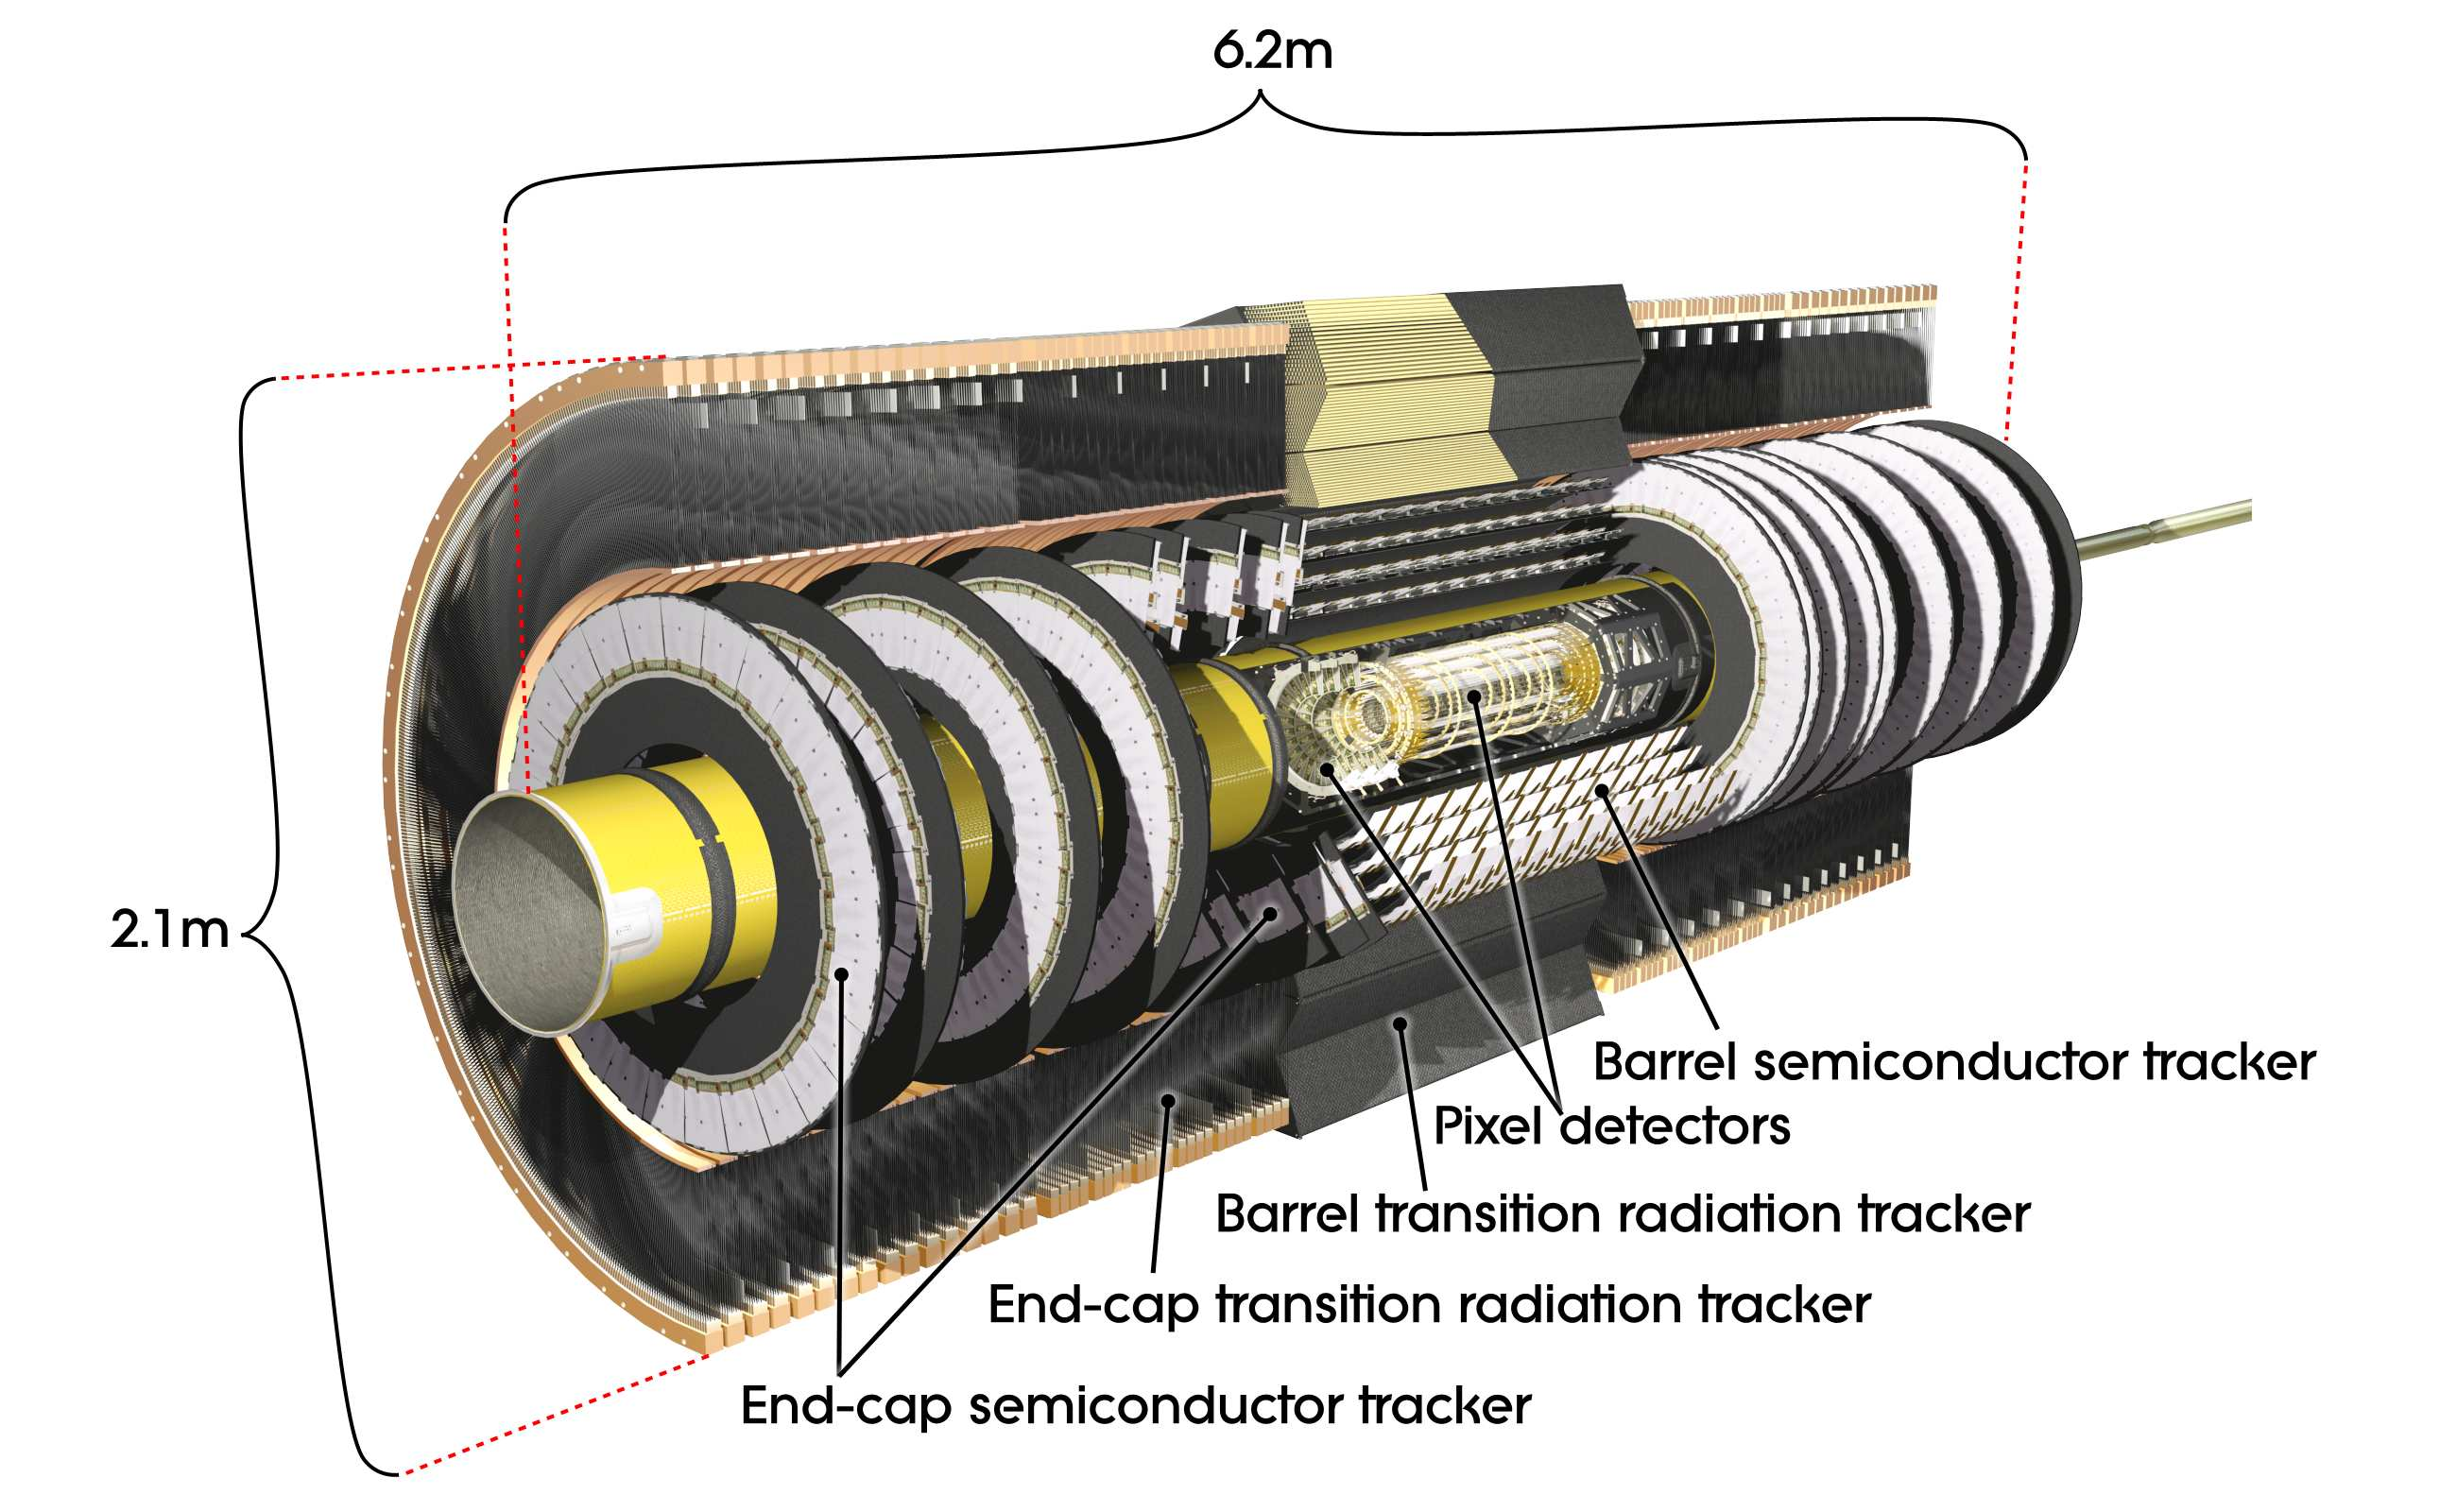
\includegraphics[width=0.8\textwidth]{figures/Detector/ID_newTRT_d3.png}
  \caption{Schematic diagram of the ATLAS inner detector\cite{Aad:1698966}.}
  \label{fig:inner_dec}
\end{figure}

%% ============================== Pixel detector ====================================
\textbf{Pixel detector}

The pixel detector~\cite{pixel_2008} is the innermost part of ATLAS tracking system.
With finest granularity of materials, it has the best spatial resolution and 3-dimensional space-point measurement in inner detector.
ATLAS Pixel Detector for the LHC run-2 is composed of 4 layers of barrel pixel detector and two end-caps with three pixel disks each, as shown in figure~\ref{fig:inner_pixel}.
There are three outer layers that originally installed for run-1 and one additional layer called Insertable B-Layer (IBL) that newly constructed in run-2~\cite{Mullier:2016}.
Now the 4-layer pixel detector has very good reconstruction of primary and secondary vertices, which is even crucial for long-lived particles like $\tau$-lepton and b-quark.
\begin{figure}[!htb]
  \centering
  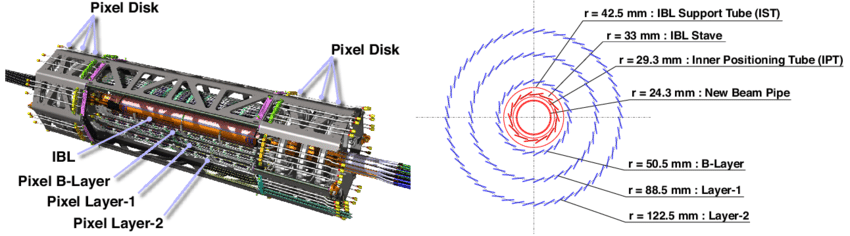
\includegraphics[width=1.0\textwidth]{figures/Detector/inner_pixel.png}
  \caption{Schematic diagram of the ATLAS 4-Layer Pixel Detector.}
  \label{fig:inner_pixel}
\end{figure}

%% ================================ SCT ===========================================
\textbf{Semiconductor Tracker}

The Semiconductor Tracker (SCT)~\cite{SCT_2007} installed outside the pixel detector is the middle component of the inner detector.
It has similar function as pixel detector but with long and narrow strips instead of small pixels, which makes a much larger coverage than pixel detector.
The SCT consists of 4088 modules, and contains four concentric layers in barrel (2112 modules) and nine disks in each of the two end-caps (1976 modules) as shown in figure~\ref{fig:inner_sct}.
And it measures particles over a large area with 6.3 million readout channels and a total area of 61 square meters.
The SCT is the most critical part of the inner detector for 2D track hit reconstruction.
In barrel, the hit precision is 17 $\mu$m in the \textit{r}-$\phi$ coordinate and 580 $\mu$m in \textit{z} coordinate.
In end-caps, the prevision is 17 $\mu$m in the \textit{z}-$\phi$ coordinate and 580 $\mu$m in \textit{r} coordinate.
\begin{figure}[!htb]
  \centering
  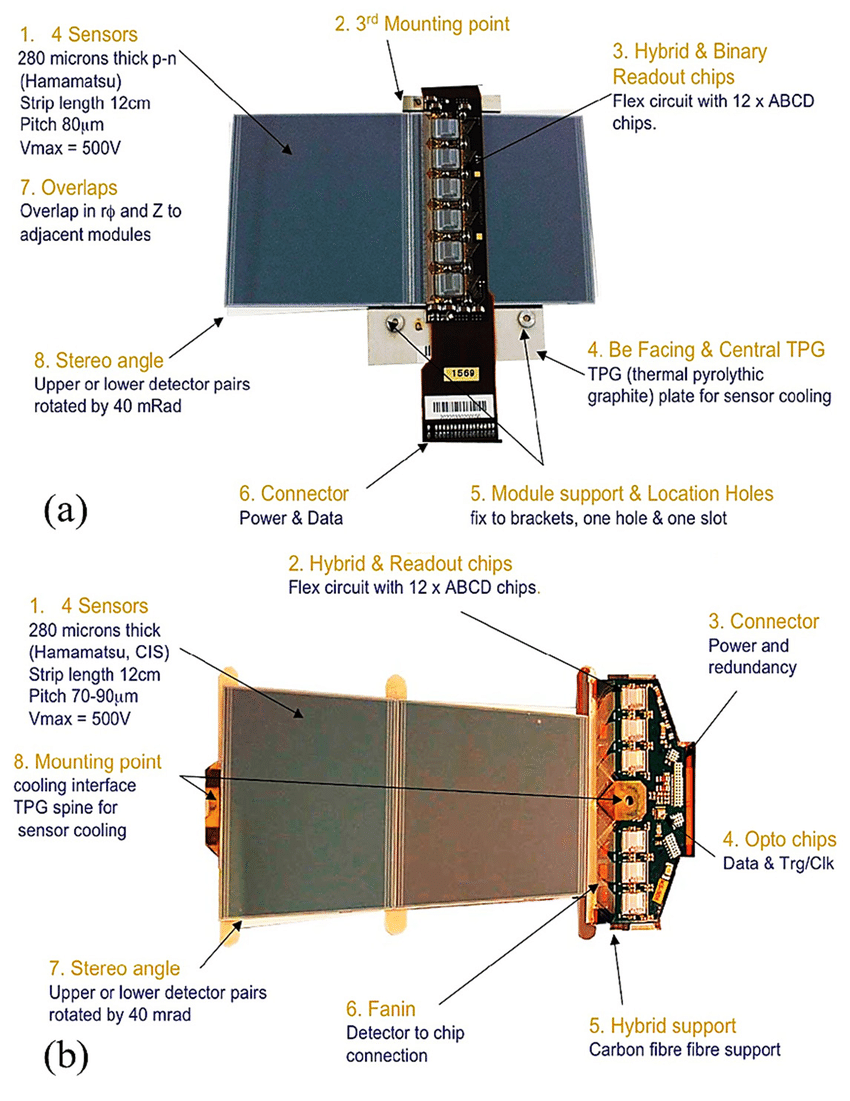
\includegraphics[width=0.8\textwidth]{figures/Detector/inner_SCT.png}
  \caption{SCT (a) barrel module and (b) end-cap\cite{Sultan:phdthesis}.}
  \label{fig:inner_sct}
\end{figure}

%% ================================= TRT ======================================
\textbf{Transition radiation tracker}

The transition radiation tracker (TRT)\cite{TRT_2008} is the outermost part of inner detector, which has a very different design comparing to the two previously sub-detectors.
It can be separated into three parts: one barrel and two end-cap regions with the $|\eta|$ coverage up to 2.0.
There are 73 barrel layers and 224 end-cap layers (112 in each) with 372000 straws in total, and about 351000 readout channels for TRT.
The TRT provides better \textit{z} resolution but much worse \textit{r}-$\phi$ resolution (about 130 $\mu$m) comparng to the pixel detector and SCT per straw.
But the straw hits still make significant contributions to momentum measurement, since its lower precision per point (compared to silicon) can be compensated by the large number of measurements and long track length.
